\documentclass[tikz,border=4pt]{standalone}
\usepackage[utf8]{inputenc}\usepackage[T1]{fontenc}\usepackage{helvet}\renewcommand{\familydefault}{\sfdefault}
\usetikzlibrary{arrows.meta}
\definecolor{faws}{HTML}{FFF2CC}\definecolor{daws}{HTML}{D6B656}
\definecolor{fdelta}{HTML}{DAE8FC}\definecolor{ddelta}{HTML}{6C8EBF}
\definecolor{fjob}{HTML}{D5E8D4}\definecolor{djob}{HTML}{82B366}
\definecolor{flocal}{HTML}{F5F5F5}\definecolor{dlocal}{HTML}{666666}
\definecolor{fquery}{HTML}{E1D5E7}\definecolor{dquery}{HTML}{9673A6}
\definecolor{fframe}{HTML}{FFFFFF}\definecolor{dframe}{HTML}{888888}
\begin{document}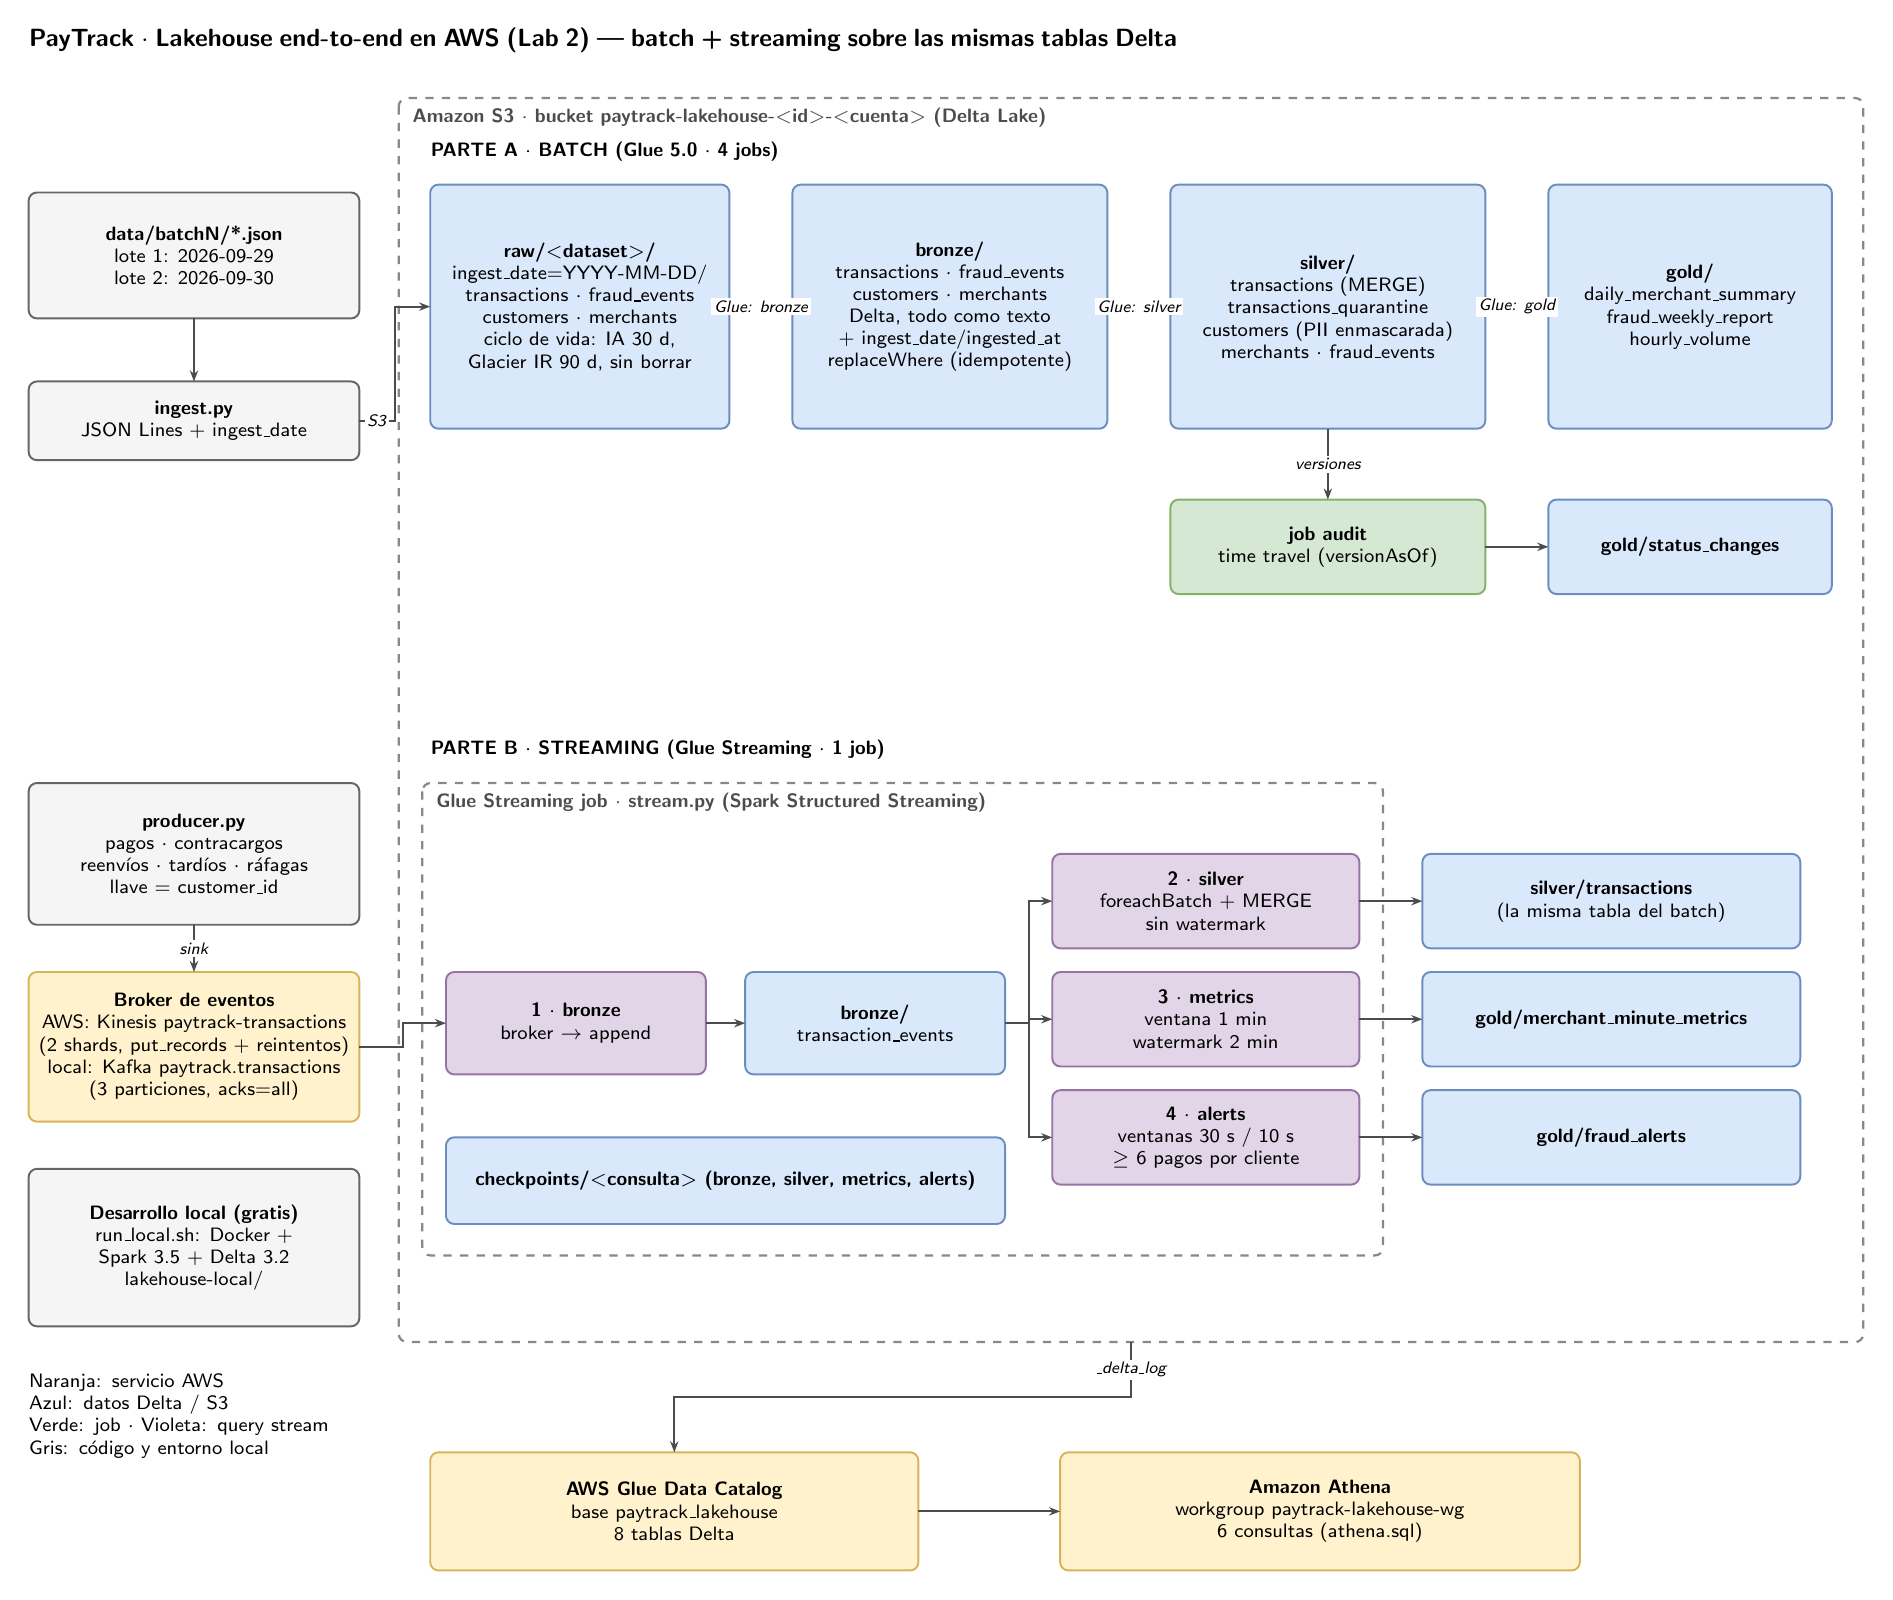
\begin{tikzpicture}[x=1cm,y=-1cm,font=\fontsize{6.8}{8}\selectfont]
\node[anchor=north west,align=left,text width=22cm,inner sep=0] (t_title) at (0.3,0.1) {\fontsize{9}{10}\selectfont\textbf{PayTrack $\cdot$ Lakehouse end-to-end en AWS (Lab 2) — batch + streaming sobre las mismas tablas Delta}};
\draw[dashed,thick,draw=dframe,rounded corners=3pt] (5.0,1.0) rectangle (23.6,16.8) coordinate(f_s3n);
\node[anchor=north west,inner sep=2pt,font=\fontsize{7}{8}\selectfont\bfseries,text=black!70] at (5.1,1.05) {Amazon S3 $\cdot$ bucket paytrack-lakehouse-\textless{}id\textgreater{}-\textless{}cuenta\textgreater{} (Delta Lake)};
\coordinate (f_s3) at (14.3,8.9);
\node[anchor=north west,align=left,text width=6cm,inner sep=0] (t_a) at (5.4,1.55) {\textbf{PARTE A $\cdot$ BATCH (Glue 5.0 $\cdot$ 4 jobs)}};
\node[anchor=north west,align=left,text width=8cm,inner sep=0] (t_b) at (5.4,9.15) {\textbf{PARTE B $\cdot$ STREAMING (Glue Streaming $\cdot$ 1 job)}};
\node[draw=dlocal,fill=flocal,rounded corners=3pt,line width=0.7pt,minimum width=4.2cm,minimum height=1.6cm,align=center,inner sep=2pt] (files) at (2.4,3.0) {\textbf{data/batchN/*.json}\\lote 1: 2026-09-29\\lote 2: 2026-09-30};
\node[draw=dlocal,fill=flocal,rounded corners=3pt,line width=0.7pt,minimum width=4.2cm,minimum height=1.0cm,align=center,inner sep=2pt] (ingest) at (2.4,5.1) {\textbf{ingest.py}\\JSON Lines + ingest\_date};
\node[draw=ddelta,fill=fdelta,rounded corners=3pt,line width=0.7pt,minimum width=3.8cm,minimum height=3.1cm,align=center,inner sep=2pt] (raw) at (7.300000000000001,3.6500000000000004) {\textbf{raw/\textless{}dataset\textgreater{}/}\\ingest\_date=YYYY-MM-DD/\\transactions $\cdot$ fraud\_events\\customers $\cdot$ merchants\\ciclo de vida: IA 30 d,\\Glacier IR 90 d, sin borrar};
\node[draw=ddelta,fill=fdelta,rounded corners=3pt,line width=0.7pt,minimum width=4.0cm,minimum height=3.1cm,align=center,inner sep=2pt] (bronze) at (12.0,3.6500000000000004) {\textbf{bronze/}\\transactions $\cdot$ fraud\_events\\customers $\cdot$ merchants\\Delta, todo como texto\\+ ingest\_date/ingested\_at\\replaceWhere (idempotente)};
\node[draw=ddelta,fill=fdelta,rounded corners=3pt,line width=0.7pt,minimum width=4.0cm,minimum height=3.1cm,align=center,inner sep=2pt] (silver) at (16.8,3.6500000000000004) {\textbf{silver/}\\transactions (MERGE)\\transactions\_quarantine\\customers (PII enmascarada)\\merchants $\cdot$ fraud\_events};
\node[draw=ddelta,fill=fdelta,rounded corners=3pt,line width=0.7pt,minimum width=3.6cm,minimum height=3.1cm,align=center,inner sep=2pt] (gold) at (21.400000000000002,3.6500000000000004) {\textbf{gold/}\\daily\_merchant\_summary\\fraud\_weekly\_report\\hourly\_volume};
\node[draw=djob,fill=fjob,rounded corners=3pt,line width=0.7pt,minimum width=4.0cm,minimum height=1.2cm,align=center,inner sep=2pt] (audit) at (16.8,6.699999999999999) {\textbf{job audit}\\time travel (versionAsOf)};
\node[draw=ddelta,fill=fdelta,rounded corners=3pt,line width=0.7pt,minimum width=3.6cm,minimum height=1.2cm,align=center,inner sep=2pt] (changes) at (21.400000000000002,6.699999999999999) {\textbf{gold/status\_changes}};
\node[draw=dlocal,fill=flocal,rounded corners=3pt,line width=0.7pt,minimum width=4.2cm,minimum height=1.8cm,align=center,inner sep=2pt] (producer) at (2.4,10.6) {\textbf{producer.py}\\pagos $\cdot$ contracargos\\reenvíos $\cdot$ tardíos $\cdot$ ráfagas\\llave = customer\_id};
\node[draw=daws,fill=faws,rounded corners=3pt,line width=0.7pt,minimum width=4.2cm,minimum height=1.9cm,align=center,inner sep=2pt] (broker) at (2.4,13.049999999999999) {\textbf{Broker de eventos}\\AWS: Kinesis paytrack-transactions\\(2 shards, put\_records + reintentos)\\local: Kafka paytrack.transactions\\(3 particiones, acks=all)};
\draw[dashed,thick,draw=dframe,rounded corners=3pt] (5.3,9.7) rectangle (17.5,15.7) coordinate(f_jobn);
\node[anchor=north west,inner sep=2pt,font=\fontsize{7}{8}\selectfont\bfseries,text=black!70] at (5.3999999999999995,9.75) {Glue Streaming job $\cdot$ stream.py (Spark Structured Streaming)};
\coordinate (f_job) at (11.399999999999999,12.7);
\node[draw=dquery,fill=fquery,rounded corners=3pt,line width=0.7pt,minimum width=3.3cm,minimum height=1.3cm,align=center,inner sep=2pt] (q1) at (7.25,12.75) {\textbf{1 $\cdot$ bronze}\\broker $\rightarrow$ append};
\node[draw=ddelta,fill=fdelta,rounded corners=3pt,line width=0.7pt,minimum width=3.3cm,minimum height=1.3cm,align=center,inner sep=2pt] (events) at (11.05,12.75) {\textbf{bronze/}\\transaction\_events};
\node[draw=dquery,fill=fquery,rounded corners=3pt,line width=0.7pt,minimum width=3.9cm,minimum height=1.2cm,align=center,inner sep=2pt] (q2) at (15.25,11.2) {\textbf{2 $\cdot$ silver}\\foreachBatch + MERGE\\sin watermark};
\node[draw=dquery,fill=fquery,rounded corners=3pt,line width=0.7pt,minimum width=3.9cm,minimum height=1.2cm,align=center,inner sep=2pt] (q3) at (15.25,12.7) {\textbf{3 $\cdot$ metrics}\\ventana 1 min\\watermark 2 min};
\node[draw=dquery,fill=fquery,rounded corners=3pt,line width=0.7pt,minimum width=3.9cm,minimum height=1.2cm,align=center,inner sep=2pt] (q4) at (15.25,14.2) {\textbf{4 $\cdot$ alerts}\\ventanas 30 s / 10 s\\$\geq$ 6 pagos por cliente};
\node[draw=ddelta,fill=fdelta,rounded corners=3pt,line width=0.7pt,minimum width=4.8cm,minimum height=1.2cm,align=center,inner sep=2pt] (o_silver) at (20.4,11.2) {\textbf{silver/transactions}\\(la misma tabla del batch)};
\node[draw=ddelta,fill=fdelta,rounded corners=3pt,line width=0.7pt,minimum width=4.8cm,minimum height=1.2cm,align=center,inner sep=2pt] (o_metric) at (20.4,12.7) {\textbf{gold/merchant\_minute\_metrics}};
\node[draw=ddelta,fill=fdelta,rounded corners=3pt,line width=0.7pt,minimum width=4.8cm,minimum height=1.2cm,align=center,inner sep=2pt] (o_alert) at (20.4,14.2) {\textbf{gold/fraud\_alerts}};
\node[draw=ddelta,fill=fdelta,rounded corners=3pt,line width=0.7pt,minimum width=7.1cm,minimum height=1.1cm,align=center,inner sep=2pt] (ckpt) at (9.149999999999999,14.75) {\textbf{checkpoints/\textless{}consulta\textgreater{} (bronze, silver, metrics, alerts)}};
\node[draw=daws,fill=faws,rounded corners=3pt,line width=0.7pt,minimum width=6.2cm,minimum height=1.5cm,align=center,inner sep=2pt] (catalog) at (8.5,18.95) {\textbf{AWS Glue Data Catalog}\\base paytrack\_lakehouse\\8 tablas Delta};
\node[draw=daws,fill=faws,rounded corners=3pt,line width=0.7pt,minimum width=6.6cm,minimum height=1.5cm,align=center,inner sep=2pt] (athena) at (16.7,18.95) {\textbf{Amazon Athena}\\workgroup paytrack-lakehouse-wg\\6 consultas (athena.sql)};
\node[draw=dlocal,fill=flocal,rounded corners=3pt,line width=0.7pt,minimum width=4.2cm,minimum height=2.0cm,align=center,inner sep=2pt] (dev) at (2.4,15.6) {\textbf{Desarrollo local (gratis)}\\run\_local.sh: Docker +\\Spark 3.5 + Delta 3.2\\lakehouse-local/};
\node[anchor=north west,align=left,text width=4.6cm,inner sep=0] (legend) at (0.3,17.2) {Naranja: servicio AWS\\Azul: datos Delta / S3\\Verde: job $\cdot$ Violeta: query stream\\Gris: código y entorno local};
\draw[-{Stealth[length=4pt]},thick,draw=black!70] (2.40,3.80) -- (2.40,4.60);
\draw[-{Stealth[length=4pt]},thick,draw=black!70] (4.50,5.10) -- (4.95,5.10) -- (4.95,3.65) -- (5.40,3.65);
\node[font=\fontsize{6}{7}\selectfont\itshape,fill=white,inner sep=1pt] at (4.72,5.10) {S3};
\draw[-{Stealth[length=4pt]},thick,draw=black!70] (9.20,3.65) -- (10.00,3.65);
\node[font=\fontsize{6}{7}\selectfont\itshape,fill=white,inner sep=1pt] at (9.60,3.65) {Glue: bronze};
\draw[-{Stealth[length=4pt]},thick,draw=black!70] (14.00,3.65) -- (14.80,3.65);
\node[font=\fontsize{6}{7}\selectfont\itshape,fill=white,inner sep=1pt] at (14.40,3.65) {Glue: silver};
\draw[-{Stealth[length=4pt]},thick,draw=black!70] (18.80,3.65) -- (19.60,3.65);
\node[font=\fontsize{6}{7}\selectfont\itshape,fill=white,inner sep=1pt] at (19.20,3.65) {Glue: gold};
\draw[-{Stealth[length=4pt]},thick,draw=black!70] (16.80,5.20) -- (16.80,6.10);
\node[font=\fontsize{6}{7}\selectfont\itshape,fill=white,inner sep=1pt] at (16.80,5.65) {versiones};
\draw[-{Stealth[length=4pt]},thick,draw=black!70] (18.80,6.70) -- (19.60,6.70);
\draw[-{Stealth[length=4pt]},thick,draw=black!70] (2.40,11.50) -- (2.40,12.10);
\node[font=\fontsize{6}{7}\selectfont\itshape,fill=white,inner sep=1pt] at (2.40,11.80) {sink};
\draw[-{Stealth[length=4pt]},thick,draw=black!70] (4.50,13.05) -- (5.05,13.05) -- (5.05,12.75) -- (5.60,12.75);
\draw[-{Stealth[length=4pt]},thick,draw=black!70] (8.90,12.75) -- (9.40,12.75);
\draw[-{Stealth[length=4pt]},thick,draw=black!70] (12.70,12.75) -- (13.00,12.75) -- (13.00,11.20) -- (13.30,11.20);
\draw[-{Stealth[length=4pt]},thick,draw=black!70] (12.70,12.75) -- (13.00,12.75) -- (13.00,12.70) -- (13.30,12.70);
\draw[-{Stealth[length=4pt]},thick,draw=black!70] (12.70,12.75) -- (13.00,12.75) -- (13.00,14.20) -- (13.30,14.20);
\draw[-{Stealth[length=4pt]},thick,draw=black!70] (17.20,11.20) -- (18.00,11.20);
\draw[-{Stealth[length=4pt]},thick,draw=black!70] (17.20,12.70) -- (18.00,12.70);
\draw[-{Stealth[length=4pt]},thick,draw=black!70] (17.20,14.20) -- (18.00,14.20);
\draw[-{Stealth[length=4pt]},thick,draw=black!70] (14.30,16.80) -- (14.30,17.50) -- (8.50,17.50) -- (8.50,18.20);
\node[font=\fontsize{6}{7}\selectfont\itshape,fill=white,inner sep=1pt] at (14.30,17.15) {\_delta\_log};
\draw[-{Stealth[length=4pt]},thick,draw=black!70] (11.60,18.95) -- (13.40,18.95);
\end{tikzpicture}\end{document}